\documentclass[12pt,a4paper,openany]{book}
%\documentclass[12pt,a4paper]{book}
\newcommand\tab[1][1cm]{\hspace*{#1}}
\usepackage{amsmath,amsthm,amssymb,graphicx,hyperref}
\usepackage[left=1.2in,right=1.2in,top=1in,bottom=1in]{geometry}
\usepackage[english]{babel}
\usepackage{xcolor}
\usepackage{float}
\usepackage[style=ieee]{biblatex}
\usepackage{csquotes}
%\bibliography{Bibliography}
\addbibresource{Bibliography.bib}
\usepackage{paralist}
\usepackage{listings}
\usepackage{multirow}
\usepackage{multicol}
\usepackage[font={bf},labelfont=bf]{caption}
\RequirePackage{hyphenat}
\usepackage{algorithmic, algorithm}
\usepackage[inline]{enumitem}
\newtheorem{thm}{Theorem}[section]
\newtheorem{lem}[thm]{Lemma}
\theoremstyle{definition}
\newtheorem{defn}{Definition}[section]
\theoremstyle{remark}
\newtheorem{rem}{Remark}[section]
\newtheorem{exmp}{Example}[section]
\usepackage{color}
\definecolor{light-gray}{gray}{0.80}
%\DeclareUnicodeCharacter{0301}{*************************************}

\renewcommand{\lstlistingname}{Figure}% Listing -> Figure

\makeatletter
\AtBeginDocument{%
  \let\c@figure\c@lstlisting
  \let\thefigure\thelstlisting
  \let\ftype@lstlisting\ftype@figure % give the floats the same precedence
}
\makeatother

\makeatletter
\renewcommand*{\ext@figure}{lot}
\let\c@figure\c@table
\let\ftype@figure\ftype@table
\let\listoftableandfigures\listoftables
\renewcommand*\listtablename{Tables and Figures}
\makeatother

% https://tex.stackexchange.com/questions/334246/what-does-the-phrase-underfull-hbox-badness-10000-in-paragraph-actually-mea <-----
% name figure xxx and refer to them by their no. instead of "below..."

% https://www.researchgate.net/profile/Andrew-Sung-4/publication/4115464_Static_Analyzer_of_Vicious_Executables_SAVE/links/542191cc0cf274a67fea9972/Static-Analyzer-of-Vicious-Executables-SAVE.pdf   download it as it will be useful.

% https://ieeexplore.ieee.org/abstract/document/6045967  very good idea to mention later (trustworthiness of websites checked through SCA)



\begin{document}

\sloppy

\thispagestyle{empty}
\begin{center}
\begin{figure}[h!]
\vspace{-20pt}
\begin{center}

\includegraphics[width=100pt]{FMI-03.png}
\end{center}
\end{figure}


{\large{\bf WEST UNIVERSITY OF TIMI\c SOARA

FACULTY OF MATHEMATICS AND COMPUTER SCIENCE

BACHELOR/MASTER STUDY PROGRAM:  Computer Science in English}}

\vspace{120pt}
{\huge {\bf BACHELOR THESIS}}

\vspace{160pt}
\end{center}

{\large\noindent{\bf SUPERVISOR:
\hspace{172pt} GRADUATE: }

\noindent Lect. Dr. Adrian Spătaru \hfill 
\noindent  Armand-Alexandru Balint
}

\vfill
\begin{center}
{\bf TIMI\c SOARA

2023}
\end{center}
\newpage
\thispagestyle{empty}
\begin{center}
{\large{\bf WEST UNIVERSITY OF TIMI\c SOARA
		
FACULTY OF MATHEMATICS AND COMPUTER SCIENCE
		
BACHELOR/MASTER STUDY PROGRAM:  Computer Science in English}}

\vspace{200pt}
{\huge {\bf Exploring and assessing the efficacy of Static Code Analysis }}
%Threat Detection by Static Code Checking
\vspace{153pt}
\end{center}

{\large\noindent{\bf SUPERVISOR:\hfill GRADUATE:}

\noindent Prof. Adrian Spataru\hfill
\noindent Armand-Alexandru Balint}
 

\vfill
\begin{center}
{\bf TIMI\c SOARA

2023}
\end{center}

\newpage
\normalsize{}
\vspace*{\fill}
\vspace{-2cm}
\begin{center}
\section*{Abstract}
\vspace{50pt}
\end{center}


\noindent This thesis delves into three different use cases of Static Code Analysis tools (SCA for short). The first use case of such tools would be to improve general code quality, whereas the second and third refer to investigating their efficiency in detecting vulnerabilities and respectively threatening apps by acting as an antivirus replacement. Each stage of this analysis will be examined in detail, highlighting key aspects and features by providing insights for the reader.\\

\noindent To further enhance the quality of this analysis, a few groups of differently-skilled programmers from diverse backgrounds have been asked to participate in a study where they will have to put their knowledge to the test and differentiate vulnerabilities from secure code through simple code snippets. By comparing the performance of the SCA tools with the previously-mentioned input, this study aims to provide a thorough examination of the effectiveness of these tools in practical scenarios and whether or not it is advised to use them. The different criteria for testing will be defined prior to every results showcase and the conclusive thoughts will be done based on that. \\

\noindent Through a series of comparisons between tools and humans, this thesis seeks to determine whether or not SCA tools are worth using, or if the expertise of a human combined with common sense is sufficient for effective software development. 

\vspace*{\fill}

\newpage
\normalsize{}
%%%%%%%%%%%%%%%%%%%%%%%%%%%%%%%%%%%%%%%%%%%%%%%%%%%%
%%%%%%%%%%%% cap: acknowledgements %%%%%%%%%%%%%%%%%
%%%%%%%%%%%%%%%%%%%%%%%%%%%%%%%%%%%%%%%%%%%%%%%%%%%%


\vspace*{\fill}

\vspace{-2cm}
\begin{center}
    \section*{Acknowledgements}
\end{center}

\bigskip
\bigskip
\bigskip

% \noindent To begin with, I would like to express my gratitude towards my thesis advisor Adrian Spataru for their support throughout the course of my research, providing information whenever needed and offering advice upon reaching a roadblock. Subsequently, Prof. Werner Ravyse has also provided great guidance on the scope of academic writing and on the approach of this paper over the issues mentioned.\\

% \medskip

% \noindent Furthermore, I would like to extend my thank yous to the people that volunteered to put their knowledge in the field of code vulnerabilities to the test and participate in the form that has been used to compare different Static Code Analysis tools to AI and to Humans. Without their help, I would not have been able to come across such interesting results and as a consequence, the paper wouldn't have showcased so many statistics and potentially useful information for the readers.




\noindent To begin with, I would like to express my sincerest gratitude towards my thesis advisor Adrian Spataru for his support throughout the course of my research, providing great guidance, knowledge, and resources that have been of great aid and helped me navigate through the complexities of my research topic. Subsequently, I would like to acknowledge the contributions of Prof. Werner Ravyse whom I have met during my exchange studies in Finland. His input and feedback have been of great value in refining the scope of the paper together with them addressing some of the inconsistencies presented in my research.\\

\medskip

\noindent Conclusively, I would like to extend my gratitude to the individuals that have volunteered to participate in my research study. Their willingness of sharing their expertise and knowledge in the field of code vulnerabilities has made it possible to come up with interesting, yet relevant, results; results that I believe will bring value to future industry practitioners.



\vspace*{\fill}
\tableofcontents

%\counterwithout{table}{chapter}
%\counterwithout{figure}{chapter}

\renewcommand{\listtablename}{Figures and Tables}
\listoftables

\renewcommand\lstlistlistingname{Code Snippets}
\lstlistoflistings




%%%%%%%%%%%%%%%%%%%%%%%%%%%%%%%%%%%%%%%%%%%%%%%%%
%%%%%%%%%%%% cap: intro %%%%%%%%%%%%%%%%%
%%%%%%%%%%%%%%%%%%%%%%%%%%%%%%%%%%%%%%%%%%%%%%%%%

\chapter{Introduction}\label{cap:intro}


\section{Motivation}\label{sect:motivation}

As technology is becoming more prominent in everyone's daily life, malicious intending people also gradually start targeting their victims through virtual means. In the field of computers, it is easier to get lost or lose track of one's senses and fall victim to these malevolent actions. This thesis takes on the incentive of verifying the competence of key-tools within a programmer's tool set and their accuracy in detecting threats. The tools in cause are categorised as Static Code Checkers and their purpose is to detect vulnerabilities, bad structure of code or any other mistakes that a programmer can make; these tools are made in order to help the users develop cleaner code, simplify their code's complexity, identifying potential vulnerabilities and lastly to attempt improving resource utilisation. There are various existing tools capable of performing such actions, however, there are not many in depth comparisons over these tools, and especially on different type of data; henceforth, my motivation is trying to determine the difference between tools in their own areas of expertise, and subsequently, in detecting threats. By doing so, conclusions will be able to be drawn in regards to which tools are most recommended or advised to use for a more multi-purpose aim.\\

\noindent To add to the above, comparisons between different tools will also be run on 2 other types of tests, in order to detect the usefulness of them and perhaps be able to tell if there are more advanced static code analysis tools available out there that can be integrated into larger scale projects. The reason for the addition of the latter is solely due to the fact that many companies have products whose source code is not particularly easy to follow, does not fit the code standards, or has possible flaws. 
%%%%%%%%%%%%%%%%%%%%%%%%%%%%%%%%%%%%%%%%%%%%%%%%%
%%%%%%%%%%%% chap: SCA %%%%%%%%%%%%%%%%%
%%%%%%%%%%%%%%%%%%%%%%%%%%%%%%%%%%%%%%%%%%%%%%%%%


\chapter{Static Code Analysis}\label{chapter:chap2}


\section{Static Code Analysis}\label{sect:Static Code Analysis}

Functional code written as an approach to solving a problem is hardly ever written on the first try. These bugs fall into a handful of known categories; be it typos, poor memory management, bad logic, or everything else surrounding them. Sometimes these errors can function properly for their specific tasks but will, eventually, hinder the rest of the application, if not completely break it in the long run. The most common ways of avoiding such errors are by analyzing the code or doing code reviews; albeit, not everyone is capable of doing that. Similarly, training someone to be able to perform such code reviews reliably is pernicious to the team and therefore, another approach needs to be taken. \newline

\noindent Usually, and even more so lately, when patterns could be found within problems, writing algorithms in order to help prevent faults is recommended. Corresponding programs do exist but they do not possess the knowledge of a human, therefore, their accuracy at spotting errors is not always the highest.





% https://core.ac.uk/download/pdf/6552448.pdf
% http://www.spinroot.com/uno/uno_short_pub.pdf.

\section{Static Code Analysis Approach}\label{sect:approach}

The approach of static code analysis applications is a low-level one; namely, they consider the code separately from any instance of execution. The way they scan for patterns depends from program to program -- some approach it from a source code perspective, whereas others go a few steps lower to the binaries of the program or its byte code, and with that, they take account of all possible interactions within the application. Each variant has some good points and bad points, therefore making it difficult to compare the different approaches and rank them. \newline

\noindent While byte code may be faster to analyze \cite{logozzo2008relative} due to the many simplifications it brings, it also brings along common cases of precision loss. To further add upon this, upon compiling, the compiler in cause may change the code in an attempt to optimize it, thus ensuing changes in the byte code from its uncompiled state and henceforth, the analyzer being unlikely to detect the new byte code. 

\section{Byte code vs Source Code}

Byte code is a set of instructions designed for efficient execution by an interpreter and is frankly hard to grasp and understand for a human. To visualize this, below you can find a comparison between a python loop that prints the numbers from 0 to 9, one per line, to the screen and its disassembled form. This was done through the python \textit{dis} library \parencite{disDocs} which  supports the analysis of CPython bytecode by disassembling it. 

%\begin{multicols}{2}
%\null \vfill
%\begin{lstlisting}[columns=fixed, basewidth=0.5em, basicstyle={\ttfamily}]
%for i in range(10):
%    print(i)
%\end{lstlisting}
%\vfill \null
%\columnbreak
%\begin{lstlisting}[columns=fixed, basewidth=0.5em, basicstyle={\ttfamily}]
%1    0 LOAD_NAME       0 (range)
%     2 LOAD_CONST      0 (10)
%     4 CALL_FUNCTION   1
%     6 GET_ITER
%  >> 8 FOR_ITER        6 (to 22)
%     10 STORE_NAME     1 (i)
%
%2    12 LOAD_NAME      2 (print)
%     14 LOAD_NAME      1 (i)
%     16 CALL_FUNCTION  1
%     18 POP_TOP
%     20 JUMP_ABSOLUTE  4 (to 8)
%
%1 >> 22 LOAD_CONST     1 (None)
%     24 RETURN_VALUE
%\end{lstlisting}
%\end{multicols}
\begin{lstlisting}[caption = Disassembled Python, columns=fixed, basewidth=0.5em, basicstyle={\ttfamily}, frame=lines]
                                1    0 LOAD_NAME       0 (range)
                                     2 LOAD_CONST      0 (10)
                                     4 CALL_FUNCTION   1
                                     6 GET_ITER
                                  >> 8 FOR_ITER        6 (to 22)
                                     10 STORE_NAME     1 (i)

for i in range(10):             2    12 LOAD_NAME      2 (print)
    print(i)                         14 LOAD_NAME      1 (i)
                                     16 CALL_FUNCTION  1
                                     18 POP_TOP
                                     20 JUMP_ABSOLUTE  4 (to 8)

                                1 >> 22 LOAD_CONST     1 (None)
                                     24 RETURN_VALUE
\end{lstlisting}

\noindent In contrast to Bytecode, source code is the type of code made in order for it to be easier understood by humans. This type of code and its level of readability varies from one programming language to another; the readability level being inversely proportional to the execution speed of the language in cause. One of the main reasons for this is the existence of memory management in low-level languages, a concept that not a lot of programmers grasp to a full extent.  \newline

% https://link.springer.com/content/pdf/10.1007/978-3-540-78791-4_14.pdf
% http://www0.cs.ucl.ac.uk/staff/m.harman/scam10.pdf


\noindent To further accompany the above-stated, source code is not understood by the computer and has to be compiled into a comprehensible set of instructions for the machine. This whole concept of having to translate a language into another before it can be executed by the machine is solid ground for drawing the conclusion that in regards to performance and execution speed, Bytecode will always be faster than Source code.%; a simple, yet needed, comprehensibility trade-off for better performance.  

% \section{Limitations}

% No algorithm nor engine is perfect, they are built with a specific intent and thus, it is hard to generalize them for other purposes than their initial. Given the scope of this paper, the limitations are about understanding the intent of the code.

% \subsection{Digital Signatures}   % add limitation mention at the beginning
% A simple and standard way of deciding whether or not something is a threat or potentially harmful behavior is through digital signatures. These digital signatures simply refer to code signing \cite{bencsath2012duqu}, a method widely used nowadays in order to mark the identity of the software creator and the integrity of the code on the software itself; therefore, if an application known for allowing others to create threats digitally signs itself, it will then be automatically detected. \\
% %which therefore will automatically spot and detect threats through a 3rd party software. 

% %\textit { ----- A great example of this would be modern anti-cheats that never fail to detect scripts and macros done through software that allow such actions.   (( do I try to fit this in? ))} \newline


% \noindent That being said, here we can picture a first limitation: A supposedly safe digital signature does not mean that the code about to be executed is trustworthy as it can not take into account the possibility of a compromised encryption key which, at its rate, can also imply compromised code.

% \subsection{Obfuscation}
% %When looking into Bytecode, variables are scant
% Code obfuscation is the process through which the programmer adds extra instructions and steps to the code without changing the final outcome of the algorithm. This is, in fact, a common way of turning readable source code into unreadable one. In addition, this will also make Bytecode harder to statically analyse. To further aid my previous claims, below you will be able to find obfuscated ways of performing standard integer computations in the C programming language through various memory and reference-based computations 



% % add examples of non obfuscated variants

% \begin{lstlisting}[caption = {Obfuscated computations}, columns=fixed, basewidth=0.5em, basicstyle={\ttfamily}, frame=lines, escapechar=!]
% !\colorbox{light-gray}{Variable Addition}!                    !\colorbox{light-gray}{Variable Subtraction}!
     
% int A(int a, int b){                  int S(int a, int b){
%     void *x = a;                         char *x = a, *y = ~b;
%     return &(b[x]);                      return &x[(int) &1[y]];
% }                                     }


% !\colorbox{light-gray}{Variable Multiplication}!              !\colorbox{light-gray}{Variable Division}!
  
% int M(int a, int b){                  int D(int a, int b){
%     typedef struct _                      typedef struct _
%     {                                      {
%         char whatever[b];                      char whatever[b];
%     } bb;                                  } bb;
%     return &((bb*)0)[a];                   return (bb*)a - (bb*)0;
% }                                      }
% \end{lstlisting}
% \vspace{10pt}
% Furthermore, constant values are everywhere in binary code. One other way to obfuscate things, as shown in \cite{moser2007limits} is replacing the load operation from the register with a set of equivalent instructions which are difficult to analyze statically. Put in another way, by creating a result through a sequence of operations that will always output the same value, one could make their code significantly harder to statically analyse. The code provided below follows a set of instructions which, at the end of its execution, will always output a bite array composed of 0s. \newpage
% \begin{lstlisting}[caption = {Obfuscated predicted output}, columns=fixed, basewidth=0.5em, basicstyle={\ttfamily}, frame=lines]
% int sameOutput()
% {
%     str anyAddress = load_any_address();
%     int predefined = generate_bit_array(anyAddress.length());
%     for (int i = 0; i < anyAddress.length(); ++i){
%         if (anyAddress[i] == '0')
%             predefined = predefined XOR 0;
%         else
%             predefined = predefined XOR 1;
%     }

%     predefined = predefined OR getSetOfOnes(anyAddress.length());
%     predefined = predefined AND getSetOfZeros(anyAddress.length());

%     return predefined;
% }
% \end{lstlisting}


% %.... code to generate a code sequence that always produces the same result through a given constant.  (( opaque constant calculation )) and through SAT solving methodologies (( 3SAT solving -- check FMSD slides )) 
% \noindent Code obfuscation is one step further than code abstraction; therefore, if the developer wishes to deliver code that is more difficult to understand by the reader, they can create abstractions of it. The reason why this only increases the difficulty for the human and not for the static analyzer is because there are no extra instructions that are being integrated into the code, and therefore, the byte code remains the case. An example of code abstraction can be seen below.

% \begin{lstlisting}[caption = {Levels of Code Abstraction}, columns=fixed, basewidth=0.5em, basicstyle={\ttfamily}, frame=lines, escapechar=!]
% !\colorbox{light-gray}{Level 0: No abstraction}!           !\colorbox{light-gray}{Level 1: Parameter abstraction}!

% void sum(float arr[], int len) {    void sum(float !\colorbox{light-gray}{P[]}!, int !\colorbox{light-gray}{P}!) { 
%     float sum = 0;                       float sum = 0;
%     int i;                               int i;
%     for (i = 0; i < len; i++);           for (i = 0; i < !\colorbox{light-gray}{P}!; i++)
%         sum += arr[i];                       sum += !\colorbox{light-gray}{P[i]}!;
%     printf("sum: %f",sum);               printf("sum: %f",sum);
% }                                    }


% !\colorbox{light-gray}{Level 2: Variable abstraction}!     !\colorbox{light-gray}{Level 3: Data type abstraction}!

% void sum(float P[], int P) {        void sum(float P[], int P) {
%     float !\colorbox{light-gray}{V}! = 0;                       !\colorbox{light-gray}{T}! V = 0;
%     int !\colorbox{light-gray}{V}!;                             !\colorbox{light-gray}{T}! V;
%     for (!\colorbox{light-gray}{V}! = 0; !\colorbox{light-gray}{V}! < P; !\colorbox{light-gray}{V}!++)          for (V = 0; V < P; V++)
%         !\colorbox{light-gray}{V}! += P[!\colorbox{light-gray}{V}!];                         V += P[V];
%     printf("sum: %f",!\colorbox{light-gray}{V}!);               printf("sum: %f",V);
% }                                   }
% \end{lstlisting}



% \newpage

% \subsection{Polymorphism and Metamorphism}
% Another limitation of static code analysis is the accuracy in spotting polymorphism and metamorphism. Polymorphism is the term used to define bits of code able to take different appearances despite them having a shared interface and in a similar way, metamorphism refers to the concept of ever-changing code such that no two compilations will have the same operations and outputs; \cite{metamorphismInC} providing a great introductory example. Moreover, an older study from 2003 proves that polymorphism and metamorphism are more unlikely to not being detected by static code analysis software and neither by other commercial detection software.


% % https://www.usenix.org/event/sec03/tech/full_papers/christodorescu/christodorescu_html
% % https://auto.tuwien.ac.at/~chris/research/doc/acsac07_limits.pdf !!!
% % https://crysys.hu/publications/files/BencsathPBF12eurosec.pdf
% % https://www.differencebetween.com/difference-between-source-code-and-vs-bytecode/
% % https://blog.hcltechsw.com/appscan/bytecode-compiled-vs-source-code-scanning/
% % underpinning

\section{Tools}\label{sect:tools}
In regards to tools performing static code analysis, there are a lot of options, each having their own capabilities and some performing better in some areas than others. While they achieve their intended purpose, some may fail at persistently correcting or warning the programmer of their possible mistakes in a constant manner. Moreover, they can prompt the user to some "false positives", which are basically sequences of code handled well that trigger a flag in the software to make it believe the code was handled poorly; and this is not a desired outcome that the user would want to encounter. On the other hand however, through such tools, the standard programmer will have cleaner and more straightforward code. All things considered, below are a few recommended tools for static code checking:
\begin{itemize}
    \item Embold \newline
    As a free static code checker of critical importance in the DevOps toolchain. Its simple and easy-to-understand interface coupled with a good analysis of design patterns makes Embold a great choice for the ones in need.
    \item PVS-Studio \newline
    Alas of it offering a free trial upon request, PVS-Studio is a static code checker with a primary focus on object-oriented programming. The supported languages are C, C++, C\#, and Java.
    \item SonarQube \newline
    Unlike the previous mention, SonarQube is a more generalized tool, providing support for over 25 different programming languages. To make it even more welcoming, SonarQube offers a free community edition variant and as shown in \cite{garcia2016improved} allows the implementation of additional functionality.
    \item StyleCop \newline
    For the ones looking to get affiliated with coding conventions, StyleCop is the best alternative. It has about 150 rules, among which naming conventions, readability, and layout rules, together with many more. The only downside being the fact that StyleCop is made entirely for C\#.
    % https://www.guru99.com/best-static-code-analysis-tools.html
\end{itemize}
\noindent With these tools, the norm of each standard code review cycle should include five main phases for each developer \cite{chess2007secure}; those being:
% \begin{multicols}{2}
% \begin{figure}[h]
%     \centering
%     \caption{Static Code Review Cycle}
%     \fbox{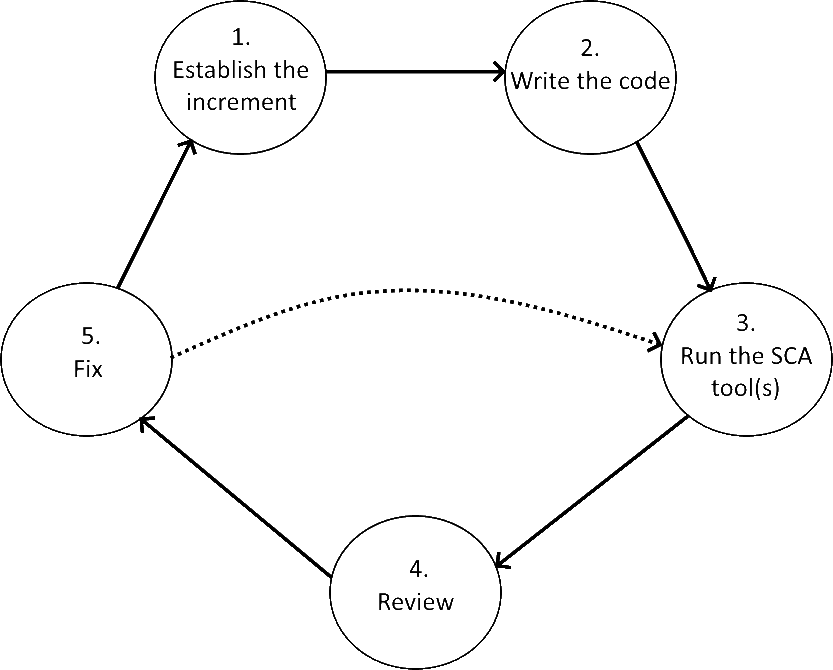
\includegraphics[scale=0.25]{./Images/SCA orderv2.png}}
% \end{figure}

% \begin{enumerate}%[vspace=0]
%     \item Establish the desired increments. Make a direction that has to be followed and draw the outline of your goal.
%     \item Write the code. Make sure that there are no lacks in the increment that is to be delivered.
%     \item Run the static code analysis tool(s).
%     \item Compare your code with the suggestions. Review the recommended changes and update the code accordingly as many times as needed
%     \item Continue the increment delivery process. 
% \end{enumerate}
% \end{multicols}

\vspace{0.6cm}
\hrule
\vspace{-0.8cm}
\begin{minipage}{0.58\textwidth}
\begin{figure}[H]
    \centering
    \caption{Static Code Review Cycle}
    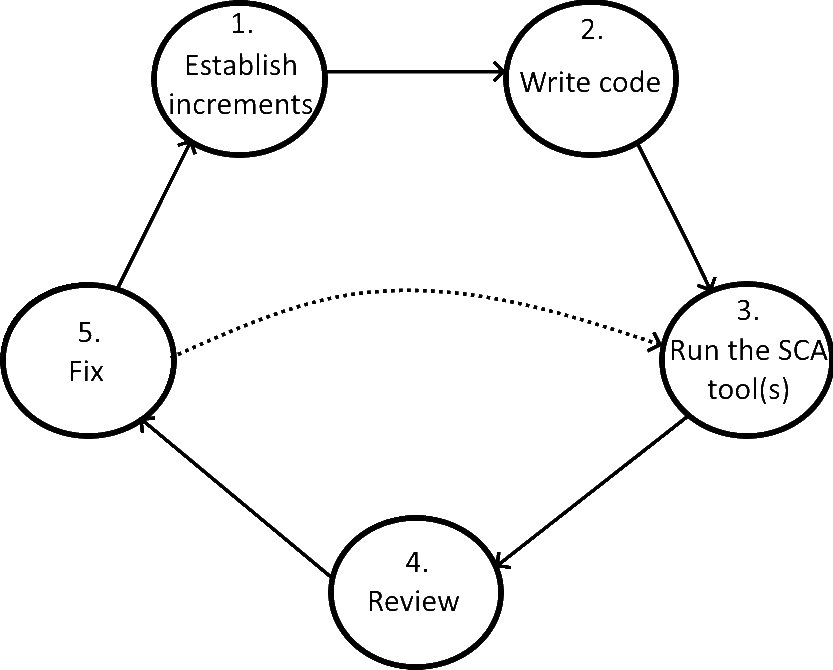
\includegraphics[scale=0.4]{./Images/sca2.png}
\end{figure}
\end{minipage}
\begin{minipage}{0.40\textwidth}\raggedleft
\vspace{1.5cm}
\begin{enumerate}%[vspace=0]
    \item Draw the outline of the new feature and establish the desired increments
    \item Write the required code for the increment
    \item Run the SCA tool(s).
    \item Compare your code with the suggestions, review the recommended changes and update the code accordingly
    \item Continue the increment delivery process. 
\end{enumerate}
\end{minipage}
\vspace{0.3cm}
\hrule

% \fbox{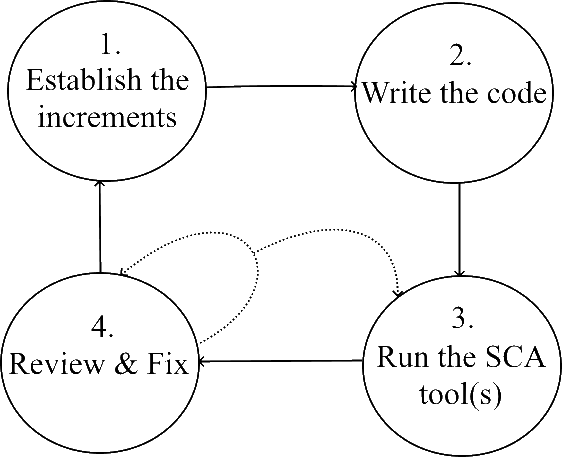
\includegraphics[]{SCA order.png}}%static code review cycle


%%%%%%%%%%%%%%%%%%%%%%%%%%%%%%%%%%%%%%%%%%%%%%%%%
%%%%%%%%%%%% cap: Threats %%%%%%%%%%%%%%%%%
%%%%%%%%%%%%%%%%%%%%%%%%%%%%%%%%%%%%%%%%%%%%%%%%%

\chapter{Benchmarks of SCA tools}\label{cap:Benchmarks}


\section{Types of tests}
In this paper, benchmarking Static Code Analysis tools will be done through multiple variations of unconventional and poorly optimized code; multiple languages will be used to expose the tools to different paradigms. The ones that will be put to the test are: Low-level memory management through C and C++, Object-Oriented via C\#, and lastly, scripting with the help of Python.\newline

\noindent To help our labeling, we will use the following table to categorize the results of each Static Code Analysis tool.

\begin{table}[htbp]
\centering
\caption{Benchmark table for code improvements}
\label{tab:SCABenchmarkTable}
\begin{tabular}{|l|llll|}
\hline
\multicolumn{1}{|c|}{\multirow{2}{*}{\textbf{\begin{tabular}[c]{@{}c@{}}Test\\ Case\end{tabular}}}} & \multicolumn{4}{c|}{Reported by tool}                                             \\
\multicolumn{1}{|c|}{}                                                                              & \multicolumn{2}{l|}{Changed} & \multicolumn{2}{l|}{Unchanged} \\ \hline
Improvable                                                                                            & \multicolumn{2}{l|}{Success}      & \multicolumn{2}{l|}{Inaccuracy}     \\ \hline
Unimprovable                                                                                            & \multicolumn{2}{l|}{Inaccuracy}     & \multicolumn{2}{l|}{Success}      \\ \hline
\end{tabular}
\end{table}

% \noindent Each possible output is composed of 2 words, the first one represents whether or not a mistake exists in the code or the code could be improved whereas the second one refers to the tool's perception of the given code.\newline

\begin{center}
    \noindent In order to compute the accuracy of the tool, the formula that will be used is:
\end{center}

\begin{equation}
100 * \frac{Successes}{Successes + Inaccuracies}    
\end{equation}\newline

\noindent The formula in cause is used to represent the correctness of the tool in regards to the tests by deducting points for wrong tool outputs and lastly, the final scoring will be multiplied by 100 in order to convert it into percentages.

% https://ieeexplore.ieee.org/abstract/document/8109084
\section{Expectations}

In regards to Static Code Analysis, it is important to catch faulty code together with improving general code quality, however, this comes as a less important factor as long as the code is functional. As research \cite{cuoq2012benchmarking} \cite{herter2019benchmarking} in the previous years have shown, Static Code Analyzers have an average detection rate of over 70\% henceforth, the most common result is expected to be \textit{Success} 

\section{Important Mentions}\label{githubRef}

The short programs and algorithms used to test the aforementioned tools are not entirely original; a part of the samples used for testing have been heavily inspired from previously seen algorithms and credits will be given where required. %On a similar note, a great amount of the samples used, if not all, will be available on GitHub in the following repository:\\
%\vspace{-15pt}
%\begin{center}
%    https://github.com/Zedpaixd/Threat-Detection-By-SCC-Thesis-samples
%\end{center}


% \subsection{Scripting}

% As a starting set of tests, a series of scripts will be used as testing data for the tools in question. These tests are meant to test the accuracy of spotting uncommon coding practices and poorly formatted code and as such, the language in which the tests will be written in, and furthermore analyzed by the tools, is Python. 



% \subsection{Memory Management}

% Moving on, in order to add one more layer of complexity to the tests, memory management will be incorporated in tests, together with references and pointers, therefore, testing the accuracy of poor memory management. Due to the incapabilities of Python to do such tasks, the tests will be written in the C language.


% \subsection{Object Oriented}

% Furthermore, in to take one more step towards abstraction, classes, inheritance, polymorphism, and method overloading will be incorporated. This serves the purpose of testing the accuracy of such tools in spotting poor program flow and bad linearity. Given the lack of such a proprietary concept in C, the language used for these algorithms will be C\#


% \subsection{General code improvements}

% Finally, as the last criterion, the testing will be done in a generalized manner; no particular testing goal but rather poorly optimized code will be used in order to determine whether or not any improvements will be found, and if so, what kind of improvements will be suggested.

\section{Results}\label{scaResults}

After running various tools over multiple code samples, it became clear that the performance of these tools has greatly improved since the previous research found in \cite{cuoq2012benchmarking} and \cite{herter2019benchmarking}. Granted that the used tools (SonarQube, PVS-Studio, StyleCop and Embold) have had similar success rates, with an average difference of 2-3\% over more than 10000 lines of code, their statistics will be averaged and the final results are as follows:

\begin{figure}[H]
    \caption{SCC results}
    \label{SCC results}
    \centering
    \includegraphics[scale=0.9]{./Images/SCC Results.png}
\end{figure}
%%%%%%%%%%%%%%%%%%%%%%%%%%%%%%%%%%%%%%%%%%%%%%%%%
%%%%%%%%%%%% cap: vulnerabilities %%%%%%%%%%%%%%%%%
%%%%%%%%%%%%%%%%%%%%%%%%%%%%%%%%%%%%%%%%%%%%%%%%%

\chapter{Vulnerabilities}\label{cap:vulnerabilities}

\section{Brief history over vulnerabilities}

Ever since the very early days of internet (cca. 1990 \cite{curran2012rethinking}), the concept of vulnerabilities started becoming of greater interest to maliciously intended programmers. Simultaneously, the rise in the popularity of software made it such that vulnerabilities became harder to spot due to the more complex nature of programs. When putting together the above-mentioned, big amounts of people started attempting to exploit the nature of these vulnerabilities. 

\section{What is a vulnerability}\label{sect:whatisavulnerability}

A vulnerability is a weakness in either the code of a software or its configuration, which can allow the exploitation of it to different extents. They can be introduced unintentionally or unwarily, due to the lack of proper testing of the program before shipping. Chances exist that these vulnerabilities can also occur in different frameworks or libraries which may be used by the developers, therefore not being introduced by them; cases similar to the Log4J incident \cite{hiesgen2022race}. 

%Vulnerabilities are weaknesses or flaws in software code, design, or configuration that can be exploited by attackers to gain unauthorized access to a system, steal data, or cause system disruption. These vulnerabilities can be unintentionally introduced during the software development process, or they may exist in third-party components used in the software.

%With the advent of the internet, software vulnerabilities became an attractive target for hackers looking to gain access to valuable data or disrupt critical systems. One of the first high-profile instances of software vulnerabilities being exploited for malicious purposes was the Morris worm in 1988. This worm, created by a graduate student, exploited vulnerabilities in Unix-based systems to spread rapidly across the internet, causing significant disruption.

%Since then, vulnerabilities have been exploited in a wide range of attacks, from the infamous SQL Slammer worm in 2003 to the Equifax data breach in 2017. The frequency and severity of these attacks have led to increased focus on vulnerability management and software security. Today, organizations use a range of tools and techniques to identify and mitigate vulnerabilities in their software, including automated scanning tools, penetration testing, and code reviews.

\section{Risks of a vulnerability}

As priorly stated, vulnerabilities pose significant risks to companies behind the software, however, not just for them; individuals are at risk too. By abusing these factors, attackers can easily gain access to various kinds of information about every user. The types of information may vary from personal ones such as payment details and sensitive conversations to more public information, such as email addresses, names or birthdays. In a similar fashion, attackers can also exploit these scenarios to execute malicious code, cause system disruption or perform denial of service attacks. Similarly, data breaches are also often caused by these vulnerabilities.

\newpage
\section{Types of vulnerabilities}

With the risks covered, there are a handful of different types of vulnerabilities that can be exploited by attackers. These different types of vulnerabilities can be classified into various kinds, and we can put them as such:
\vspace{-2px}
\subsection{Different OS Vulnerabilities}
When it comes to different Operating Systems, they tend to differ at very low levels. A simple example of this would be big-endian address storing in comparison to little-endian address storing \cite{bradley2007defining} and a visual example can be seen below:
\begin{lstlisting}[caption = {Little-endian vs Big-endian}, columns=fixed, basewidth=0.5em, basicstyle={\ttfamily}, frame=lines, escapechar=!]
  Little-endian storing          ->           Big-endian storing
   0b10010011!\colorbox{light-gray}{11111000}!           ->           0b!\colorbox{light-gray}{11111000}!10010011
\end{lstlisting}









\vspace{-2px}
\subsection{Other Software Vulnerabilities}
Moving on in the hierarchy, we have what is known as "software vulnerabilities". These occur when there are flaws in the code of a software program that can be exploited by attackers. A few prime causes of it would be improper input validation, poor memory management, incomplete error handling, poorly designed 3rd party libraries, and lack of encryption.
\vspace{-2px}
\subsection{Configuration Vulnerabilities}
Configuration vulnerabilities on the other hand may not be as self-explanatory as the prior example. These kinds of risks refer to the configuration of software and more importantly, the system that is implicitly designed to act like the hosting device for the software or website in cause. The most common faults here would be weak passwords, misconfigured permissions or rights, unnecessary open ports, and finally, unpatched systems - which simply refer to systems that are not up to date with the latest security patches and updates.
\vspace{-2px}
\subsection{Physical Vulnerabilities}
While the concept of physical vulnerabilities not being in the main scope of this paper, together with the fact that attacks have started moving virtually for a very long time now, the concept of physical vulnerabilities is still not something to be overlooked. A few common ways that may result in leaks of information are theft of physical devices, physical access to data centers and social engineering - a type of attack that involves an individual posing as something they are not, to gain information out of the victim.
\vspace{-2px}
\subsection{Human Vulnerabilities}
Finally, a great factor in the process of data theft is the victims themselves. It is taken for granted that not everyone can excel at everything, and thus, some people have a harder time understanding the things they should be wary of, henceforth putting them at risk. Some of these factors are weak passwords, trusting unknown sources, lack of security awareness, and ultimately, being easily manipulated by others. 

\section{Notable attacks in recent years}

In the past years a variety of attacks had happened, those attacks varying from small scale to larger scale and the types of weaknesses abused varying from one to another. Below a few of the bigger-scale attacks within the past few years can be seen:


\begin{itemize}
    \item \textbf{Heartbleed} OpenSSL Vulnerability - \textit{2014} \cite{durumeric2014matter} \\
    Heartbleed is a vulnerability focusing on an error within an OpenSSL cryptographic software library that allowed the attackers to access the sensitive information of victims, among which passwords and private keys could be found too. 

    \item \textbf{Dirty COW} Security Vulnerability - \textit{2016} \cite{saleel2017linux} \\
    The Dirty COW incident was a security vulnerability that affected the Linux operating system kernel; it allowed attackers to gain write access to read-only memory mappings, including files that were supposed to be protected, essentially giving them root access.

    \item \textbf{LogPetya} Ransomware Attack - \textit{2017} \cite{aidan2017comprehensive} \\
    The Attack of LogPetya started with a Microsoft Windows vulnerability called Eternal Blue which allowed code to be executed on machines running Windows 7 or older alternatives. This opportunity was used to infect computers with a virus that encrypted the user's files and demanded ransom for their recovery.

    \item \textbf{Equifax} Data Breach - \textit{2017} \cite{berghel2017equifax} \\
    The Equifax Data Breach was a vulnerability found in the web application framework provided by Apache Struts, that allowed the attackers to ascertain the personal information of over 145 million customers.

    \item \textbf{BlueBorne} Bluetooth Vulnerability - \textit{2017} \cite{seri2019exploiting} \\
    As a way of linking devices, a Bluetooth vulnerability represents a great risk for the owners of any device that is capable of using it. The creators of BlueBorne made use of the vulnerability such that they will be able to take control of a device, spread malware, or steal private data without any user awareness or interaction.

    %\item \textbf{Wannacry} Ransomware Attack - \textit{2017} \cite{mohurle2017brief} \\
    %By abusing a vulnerability in Microsoft Windows, attackers were capable of spreading their ransomware all across the globe, disrupting a great number of businesses and organizations.

    \item Apache Web Server Vulnerability - \textit{2017} \cite{kim2017vuddy} \\
    Through the abuse of a buffer overflow vulnerability in the Apache Web Server, attackers could execute arbitrary code on the affected server and ultimately steal sensitive data of the users or even cause total system disruption.

    \item Cloudflare Leak - \textit{2017} \cite{baisakhiya2017cloud} \\
    Caused by a parsing bug in Cloudflare's edge servers, one website's data would inadvertently leak into another which gave the attackers access to passwords, cookies and encryption keys of websites using Cloudflare's services.

    
\end{itemize}

%Meltdown and Spectre (2018) - Vulnerabilities in computer processors that allowed attackers to steal sensitive information, such as passwords and encryption keys.

%In conclusion, vulnerabilities in software can pose significant risks to organizations and individuals, including data theft, malware attacks, DoS attacks, and account takeover. It is important for organizations to take proactive measures to identify and mitigate vulnerabilities in their software to minimize these risks.



\section{Testing for vulnerabilities}
When testing for vulnerabilities, it's best to keep in mind that no method is fail-proof and each method has its own drawbacks which may or may not be present in other alternatives. These methods can vary from human-based to machine-reliant and their methods may vastly differ from one another. The most commonly used methods are: \cite{al2013survey}

\begin{multicols}{2}
\begin{itemize}
    \item Code Reviews
    \item Fuzz Testing
    \item Risk Analysis
    \item Penetration Testing
    \item Compliance Testing
    \item Dynamic Testing
\end{itemize}
\end{multicols}

\subsection{Code Reviews}
Code reviewing is a manual process where a security analyst, if not the programmer, inspects the source code line by line in a linear pattern to identify any potential vulnerabilities that may pose a threat to the security of the software. As some older studies have concluded, this approach is the most time-consuming and arduous out of all others, as the person reviewing the code needs to have a deep understanding of the programming language together with the security risks that are associated with it \cite{ackerman1984software,fagan2002design}.

\subsection{Fuzz Testing}
Unlike the other types of tests and ways to analyze code, Fuzz testing (also known as Fuzzing) takes a less computational path and instead makes use of scripts to inject randomly generated data into the software. The type of input and data generated are typically nonsensical and follow no rules, except for the fact that they are used for one goal in particular (such as testing API requests for example). Given how Fuzzing is based on randomness, it is not guaranteed that it will detect all different types of issues, but it will help stabilize the software, API, or any other system in case upon receiving erroneous data. 

\subsection{Risk Analysis}
Risk analysis is the process of reviewing security requirements and identifying the risks based on the requirements; this is typically carried out during the design phase of the software and is done in correlation with an assessment of the likelihood and impact of the risk, therefore determining the importance of it \cite{khan2012systematic}. One frequently used technique is Failure Mode and Effects Analysis (or FMEA for short). This is a structured approach to also identifying and evaluating potential failures in the software to then take steps and minimalize, if not fully prevent, their effects \cite{lipol2011risk}. 

\subsection{Penetration Testing}
Also known as Ethical Hacking, Penetration Testing is the process of testing the Network Security of the system or server and whether or not the system resists attacks successfully, together with how it behaves when a vulnerability is exploited. Finally, it is also a common practice for "Ethical Hackers" to attempt to exploit vulnerabilities that have priorly been detected in previous review iterations \cite{caballero2007polyglot}.

\subsection{Compliance Testing}
A recent study from 2017 explains how roughly 40\% of breaches are due to employee carelessness \cite{balozian2017review} and according to another study, about 48\% of employees lack awareness in the security domain \cite{coopers2014global}. Given that information, Compliance testing has seen an increase in usage over the past couple of years. That being said, Compliance testing is the process that aims to ensure that the software systems tested are up to the standards of specific regulations, standards and guidelines. Similarly, they are typically also verified from a UML point of view \cite{bunyakiati2009compliance} and lately the concept of test and data-driven testing increasing \cite{steffens2018towards}.

\subsection{Dynamic Testing}
Conclusively, our last alternative, Dynamic Testing, is the opposite of Static Testing. This way of testing involves running the software and observing its behaviour in real-time in order to help identify errors that are difficult to detect through other means. This technique conjoins multiple other techniques such as penetration testing and fuzz testing in order to make the process as successful in detecting vulnerabilities as possible.

\section{Vulnerability detection through SCC}
When looking for vulnerabilities in the code of a software, it is important to remind ourselves about all factors that can influence a human's thought process during a review. These factors can include, but will not limit themselves to: Mood, bias for one's own work, time pressure, environment, etc. In contrast to that, tools are objective and will always function in the way they have been programmed to - or in other words, have no emotions nor a chance to miss a threat that it has been instructed to detect. On a similar note, one other important factor that should be taken into account is time conservation. A human will take time to analyze logically the flow of the code, whereas a program can perform the same task in a matter of moments, thus increasing performance.

\section{Testing criteria}
Granted the fact that vulnerabilities are caused by aspects that have not been taken into account, if not completely overlooked by humans, the difficulty in spotting these issues will be accounted for the final score of this category too.\smallskip\\  A group of programmers with different backgrounds has been asked to review the sample codes used to test the software on, where they will first be asked if they believe that there is a vulnerability in the code and secondly, if there is indeed a vulnerability, they will be asked to add a review of how difficult it would be to spot it. The ratings for each sample will be taken into account and an average of it will be made, together with a bias for the first answer. This will determine the difficulty of spotting the specific type of vulnerability and will be used as a side comparison for the results provided by the Static Code Analysis tools. 

\subsection{Types of tests}
Given the various types of vulnerabilities, the tests will be done on the following types of vulnerabilities:
\begin{multicols}{2}
\begin{itemize}
    \item SQL Injections
    \item Authentication
    \item Buffer Overflows
    \item Unclosed Files
    \item Poor memory management
    \item Insecure deserializing
    \item Server-Side Template Injection
    \item Insecure Direct Object References
    \item Session Hijacking
    \item Poor Hashing
    \item CSRF
    \item XSS
    \item Language-Specific vulnerabilities
\end{itemize}
\end{multicols}

\noindent The code snippets used for these tests have been written by hand and ultimately tested for vulnerabilities, assuring that there would be some way to abuse it. The programming languages that were used for the testing are C, C\#, PHP, and Python; the samples are able to be found on the GitHub repository referenced in \autoref{githubRef} 

\section{Tested Tools}
Due to conventional reasons, the tools that will be tested are going to require either a free variant or at least a trial. For the rest of the tools that will be used, we can enumerate:
\begin{multicols}{2}
    \begin{itemize}
        \item SonarQube
        \item Kodezi
        \item PVS-Studio
        \item Snyk Code
        \item Codiga
    \end{itemize}
\end{multicols}

\subsection{AI in Vulnerability Detection} \label{chatgpt}
With the rise in popularity of AI in the current days, researchers are now, starting to use AI to automatically generate much more elaborate rule sets for parsing code. For example, a team of researchers at ETH Zurich is now making a similar AI tool available for mainstream adoption. And granted this information, one of the most advanced and popular tools that is here to stay \cite{kasneci2023chatgpt}, ChatGPT, will also be used as a side comparison too in order to gain a better grasp over whether or not AI has a future in Static Code Analysis.

\section{Expectations}
Granted that both tools and humans have limitations and that AI is a permanently growing tool, it would not be a surprise if AI will outperform both humans and static code checkers in detecting vulnerabilities, and if not now then in the soon future. On the other hand, out of SCA tools and Humans, it would be expected having the tools be of a higher consistency. While humans can provide valuable insight and context, they can be prone to error and may also be limited by knowledge.

\vspace{-3mm}

\section{Results} \label{VSCAResults}

\subsection{Accuracy of Tools}

Following the template of the previous tool accuracy done in \ref{scaResults}, splitting will be done based on the type of languages that these vulnerabilities have been written in, this is done due to the fact that not all tools are capable of performing just as well on all languages. That being said, these language types are Low-Level languages (C \& C++), OOP languages (C\#), and finally, Scripting languages (Python \& PHP). Cutting to the chase, the average of tools for each category is:

\vspace{0.4cm}
\hrule    
\hspace{-0.6cm}
\begin{minipage}{0.5\textwidth}
\begin{figure}[H]
    \caption{Low-Level}
    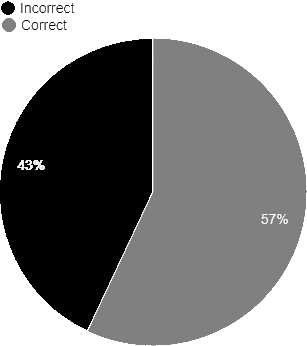
\includegraphics[scale=0.65]{./Images/VSCA low level.png}
\end{figure}
\end{minipage}
\hspace{0.8cm}
\begin{minipage}{0.45\textwidth}\raggedleft
\begin{figure}[H]
    \caption{OOP}
    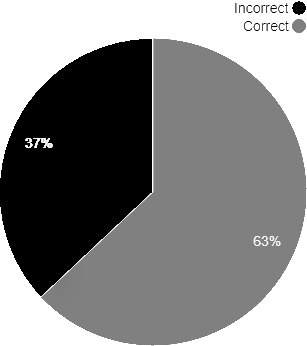
\includegraphics[scale=0.65]{./Images/VSCA OOP.png}
\end{figure}

\end{minipage}
\hspace{-0.6cm}
\begin{minipage}{0.5\textwidth}
\begin{figure}[H]
    \caption{Scripting}
    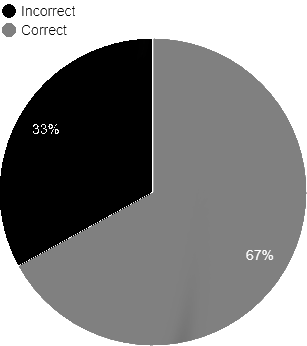
\includegraphics[scale=0.65]{./Images/VSCA scripting.png}
\end{figure}
\end{minipage}
\hspace{0.8cm}
\begin{minipage}{0.45\textwidth}\raggedleft
\begin{figure}[H]
    \caption{Median}
    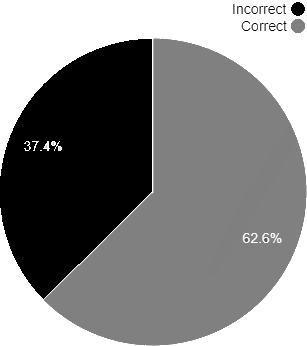
\includegraphics[scale=0.65]{./Images/VSCA avg.png}
\end{figure}

\end{minipage}
%\vspace{0.4cm}
%\hrule



\subsection{Accuracy of Humans}\label{humanacc}
\begin{center}
    With a total of 45 volunteers with different backgrounds and areas of expertise, below can be seen a graph representing their years of experience and their current field of work
\end{center}






\hrule    
\begin{figure}[H]
    \centering
    \caption{Volunteer Breakdown}
    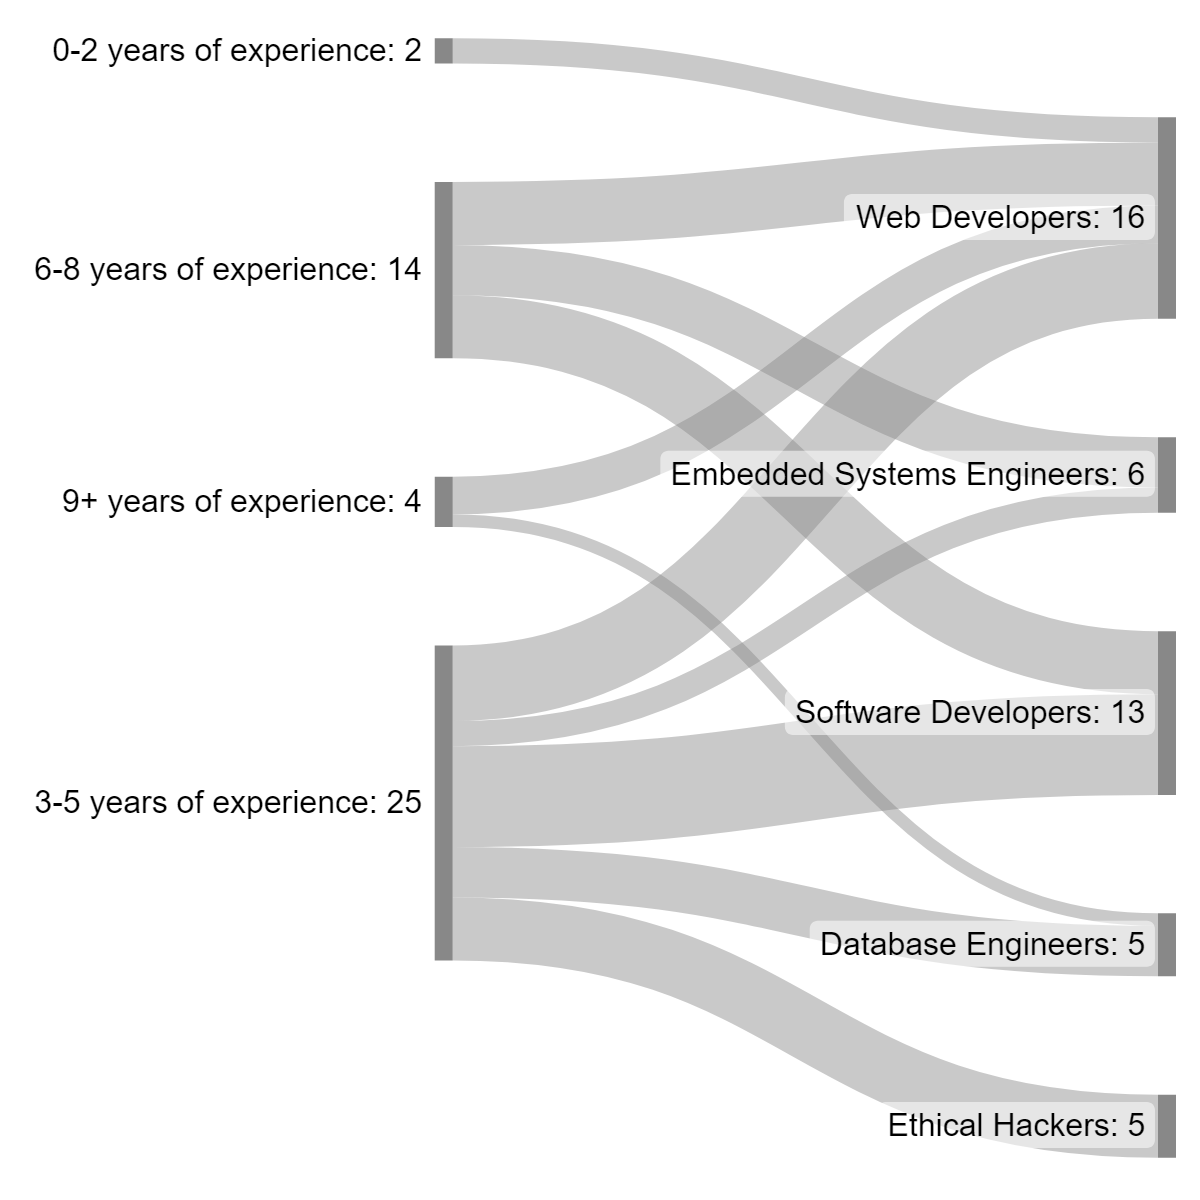
\includegraphics[scale=0.25]{./Images/breakdown.png}
\end{figure}
\hrule

\begin{center}
    And for a more detailed version of the volunteers' background and experience
\end{center}

\begin{lstlisting}[columns=fixed, basewidth=0.5em, basicstyle={\ttfamily},nolol]
Embedded Systems Engineers:             
                3-5 years - 2           Web Developers:
                6-8 years - 4                     0-2 years - 2
                                                  3-5 years - 6
   Database Engineers:                            6-8 years - 5
                3-5 years - 4                     9+  years - 3
                9+  years - 1                   
                                            
    Software Developers:                 Ethical Hackers:
                3-5 years - 8                     3-5 years - 5
                6-8 years - 5

\end{lstlisting}
\vspace{0.3cm}
\noindent The form the volunteers had to fill out provided them with 32 code snippets and asked them if there is a vulnerability present in the particular snippet. If they believe there is a vulnerability, they will then be asked to rate the difficulty of an average programmer with similar knowledge to theirs spotting the vulnerability. This rating was on a scale of 0 to 5 where 0 would be equivalent to "an obvious vulnerability" and 5 being something that will probably go under the radar, at least according to the opinion of the form-filler. In order to simplify the results, the ratings ranging from 0 to 2 will be treated as "easy to spot" and from 3 to 5 as "difficult to spot".\\

\noindent Primarily, there were 3 main types of vulnerabilities that the volunteers had to spot, each being split into multiple forms of it and in different languages. These 3 types are Back-end vulnerabilities (XSS, CSRF, Unrestricted file uploads, etc.), Overflows(Memory, Pointers, etc.), and Improper Sanitizing (SQL Injections, Paths, Direct object references, etc). For each category, a chart will be provided with the average accuracy of the volunteers and conclusively, one last for the overall standings of all categories.

\vspace{0.4cm}
\hrule    
\hspace{-0.6cm}
\begin{minipage}{0.5\textwidth}
\begin{figure}[H]
    \caption{Back-end}
    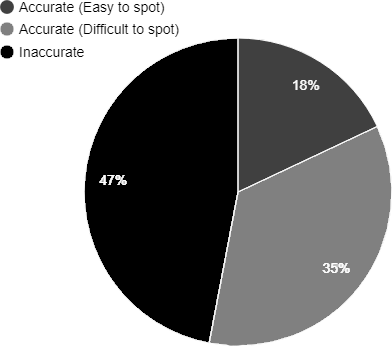
\includegraphics[scale=0.65]{./Images/web.png}
\end{figure}
\end{minipage}
\hspace{0.8cm}
\begin{minipage}{0.45\textwidth}\raggedleft
\begin{figure}[H]
    \caption{Sanitizing}
    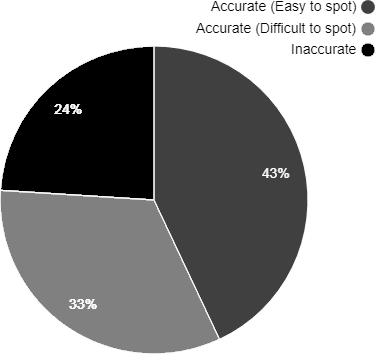
\includegraphics[scale=0.65]{./Images/unsanitized.png}
\end{figure}

\end{minipage}
\hspace{-0.6cm}
\begin{minipage}{0.5\textwidth}
\begin{figure}[H]
    \caption{Overflows}
    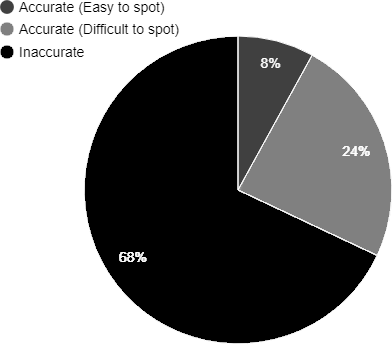
\includegraphics[scale=0.65]{./Images/overflows.png}
\end{figure}
\end{minipage}
\hspace{0.8cm}
\begin{minipage}{0.45\textwidth}\raggedleft
\begin{figure}[H]
    \caption{Median}
    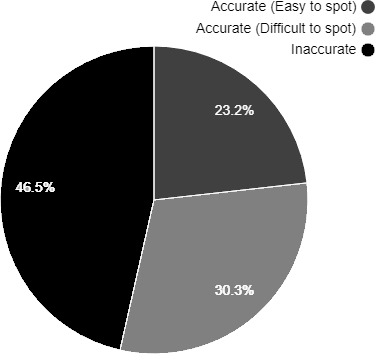
\includegraphics[scale=0.65]{./Images/avg.png}
\end{figure}

\end{minipage}
\vspace{0.4cm}
\hrule

\noindent As can be seen, on average, approximately half of the vulnerabilities went undetected by our volunteers. One thing worth mentioning is how the form presented code snippets of at most 30 lines of code, henceforth, the bias towards overlooking a possible vulnerability should go up when comparing these to production code.

% \hrule
% \vspace{-0.8cm}
% \begin{minipage}{0.58\textwidth}
% \begin{figure}[H]
%     \centering
%     \caption{Static Code Review Cycle}
%     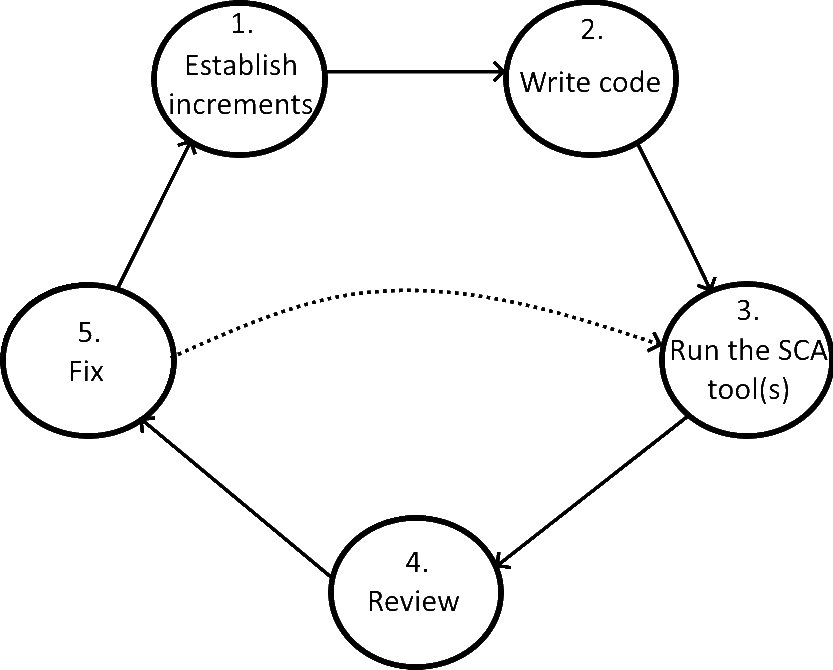
\includegraphics[scale=0.4]{./Images/sca2.png}
% \end{figure}
% \end{minipage}
% \begin{minipage}{0.40\textwidth}\raggedleft
% \vspace{1.5cm}
% \begin{figure}[H]
%     \centering
%     \caption{Static Code Review Cycle}
%     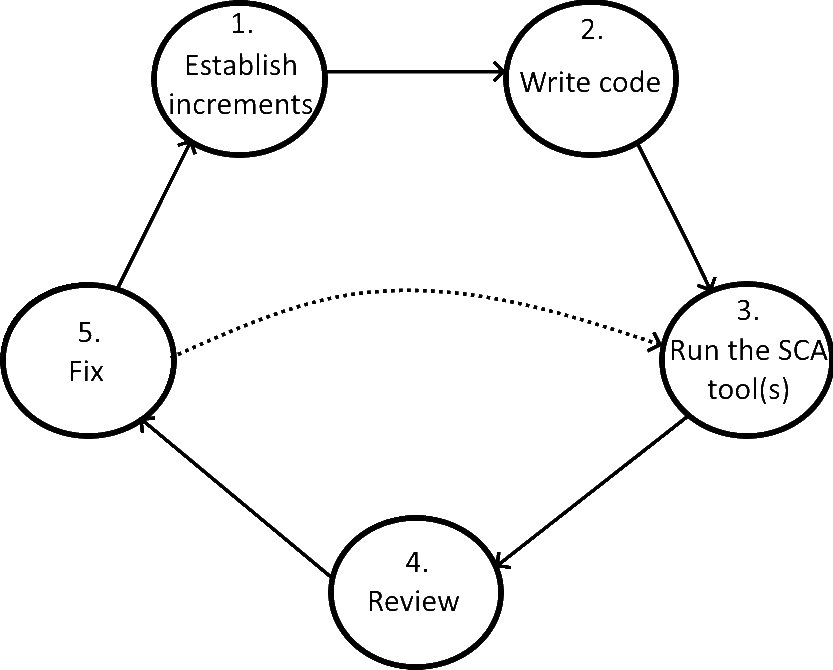
\includegraphics[scale=0.4]{./Images/sca2.png}
% \end{figure}
% \end{minipage}
% \vspace{0.3cm}
% \hrule



% 3-5 years of experience [6] Web Developers
% 6-8 years of experience [5] Web Developers
% 9+ years of experience [3] Web Developers
% 0-2 years of experience [2] Web Developers

% 3-5 years of experience [8] Software Developers
% 6-8 years of experience [5] Software Developers

% 6-8 years of experience [4] Embedded Systems Engineers
% 3-5 years of experience [2] Embedded Systems Engineers

% 3-5 years of experience [5] Ethical Hackers

% 3-5 years of experience [4] Database Engineers
% 9+ years of experience [1] Database Engineers
    
\subsection{Accuracy of AI}

As a last test in detecting vulnerabilities, ChatGPT has been asked to determine whether the code snippets provided to the responders from \ref{humanacc} contain any form of vulnerabilities, and if they do, to provide the name and solution. Upon multiple similar prompts, it became quite clear that was no consistency between the provided answers. Sometimes completely functional code would be deemed vulnerable due to too much memory management and sometimes vulnerable code would either be considered safe or as unsafe due to completely unrelated reasons, therefore making AI a very unstable resource/alternative.\\

\noindent Disregarding the above however, below can be seen the accuracy of ChatGPT in detecting the same vulnerabilities as the volunteers from the previous point after being provided a list of all possible vulnerabilities that may be encountered in the prompted code snippets. \\

\noindent\textbf{Disclaimer:} The percentages shown below may fluctuate for subsequent attempts.

%64.28\%  - 2x "partly correct" 
% C - buffer overflow: correct
% C - no file close: 			incorrect
% C - no free:                            incorrect
% C - ScanF: correct

% C# - Deserealize: partly correct
% C# - unsafe: correct
% C# - IDOR: correct
% C# - integer overflow: partly correct
% C# - integer overflow2: correct
% C# - SSTI:                               incorrect
% C# - SQL: correct
% C# - URaF: correct

% PHP - eval: correct
% PHP - include: correct
% PHP - Session Hijacking: correct
% PHP - unserialize: correct
% PHP - variable:                        	  incorrect

% PY - Bad error handling:  		  incorrect
% PY - Bad Hash: correct
% PY - BAaSM: 				  incorrect
% PY - CSRF: correct
% PY - Information leakage: correct
% PY - OS command injection: correct
% PY - Overflow: correct
% PY - Path:                		  incorrect
% PY - SQL: correct
% PY - Unrestricted file upload: 		  incorrect
% PY - XSS: 				  incorrect

% 64.28\% correct

\begin{figure}[H]
    \caption{ChatGPT Accuracy}
    \label{chatgptaccuracy}
    \centering
    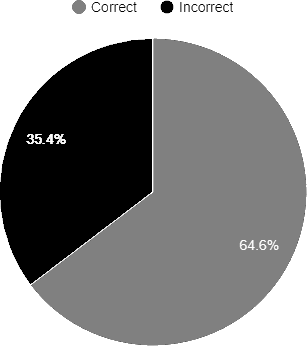
\includegraphics[scale=0.75]{./Images/chatGPT.png}
\end{figure}

\newpage
\subsection{Final Results} 

\hrule
\begin{minipage}{0.5\textwidth}
\begin{figure}[H]
    \caption{Tools}
    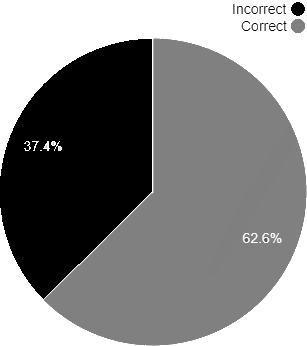
\includegraphics[scale=0.75]{./Images/VSCA avg.png}
\end{figure}
\end{minipage}
\hspace{0.8cm}
\begin{minipage}{0.45\textwidth}\raggedleft
\begin{figure}[H]
    \caption{Humans}
    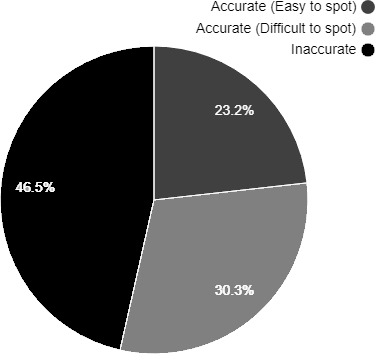
\includegraphics[scale=0.75]{./Images/avg.png}
\end{figure}

\end{minipage}
\vspace{0.4cm}
% \begin{figure}[H]
%     \caption{AI}
%     \centering
%     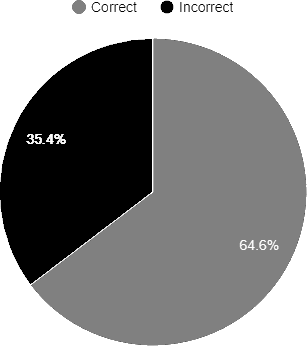
\includegraphics[scale=0.75]{./Images/chatGPT.png}
% \end{figure}
\hrule
\vspace{0.4cm}

\noindent Conclusively, in the comparison between the three for detecting vulnerabilities in code, it was found that Tools outperformed humans for smaller code snippets.
%AI was the most accurate with a success rate of 64.28\%, followed by SCA tools with a 57.85\% success rate, and lastly, humans, with a 53.5\% success rate.
While humans have a better understanding of the context and theoretical intent of the code, they are prone to making mistakes and thus this percentage may fluctuate greatly, in both directions. Tools are useful for automating repetitive tasks and can detect known patterns of errors, however, they may not be able to identify more subtle issues all the time and as such, while they seemingly outperformed the competition, they should she used as a helper rather than a guide.\\

%\subsubsection{Is AI proving itself worthy?}

\noindent And to answer the question that was opened in \ref{chatgpt}, given the results shown in Figure \ref{chatgptaccuracy}, AI has great potential in the future and if approached properly, could possibly be integrated into different SCA tools in order to drastically improve their performance and utility.
%%%%%%%%%%%%%%%%%%%%%%%%%%%%%%%%%%%%%%%%%%%%%%%%%
%%%%%%%%%%%% cap: Threats %%%%%%%%%%%%%%%%%
%%%%%%%%%%%%%%%%%%%%%%%%%%%%%%%%%%%%%%%%%%%%%%%%%

\chapter{Threats}\label{cap:threats}


\section{What is a Threat}
In real life, a threat represents a hostile action towards someone in retribution for something, either as the aftermath of another action or due to pure malicious intent. This definition translates quite accurately into the virtual world too. A virtual threat relates to the security of a device being compromised; either through the execution of a malevolent executable file or through a vulnerability found in different frameworks, libraries, etc. ultimately leading to cyber-attacks or backdoors that result in data being stolen, lost or edited. A well-known case of such incidents was the Log4j vulnerability from 2021 that affected a lot of applications resulting in an abundance of compromised data; a great in depth explanation of it can be found in \cite{hiesgen2022race}


\section{Threat Incentives}\label{sect:incentive}
The purpose behind creating a threat can be of various types, although it often seems to be linked to a desire of stealing money from preyed-upon victims. The most common practice for this is through ransomware; a type of threat that encrypts all of the user's files and targets their wallet by threatening them with the deletion of all their files if the payment is not done in due time. This is done in order to stir psychological pressure in them, henceforth losing rationality and paying the ransomware creators.%  As this topic begins to drift from ours, two good reads on this idea are \cite{noorbaloochi2015payoff} and \cite{maule2002effects}. 
\newline

\noindent An ulterior incentive of a threat is getting personal information out of the user (i.e. credentials for a website, banking account information, etc.) and this is done through keylogging. A keylogger is a type of software that records the victims' keyboard inputs together with where they are made then sends them to the attacker's database. Through this, the victim will inadvertently expose their private information and passwords, giving full access of their accounts to the creator.% A similar incentive is behind the backdoor exploiters.
\newline

\noindent And finally, the last common motive is the creation of a botnet. This refers to a network of computers infected by malware that are then put under the control of the attacking party. Each device included in this network can be commanded simultaneously to conduct a coordinated attack. These can be spread in many ways but the most common way is through email (similar to the ILOVEYOU virus \cite{knight2000iloveyou}). A well known botnet threat is the Conficker virus \cite{kaskaconficker}, also known as Downadup, a threat created in 2008 that has infected millions of Windows computers since and caused damages worth approximately \$9 billion.


\section{Types of threats}\label{chap:threattypes}
In order to fulfill their goals, the threat developers take different approaches and go to great lengths, henceforth, multiple types of threats have been created. Given the large density of them, they have been given the name of "malware" (or "malicious software" in other words) in order to categorize them all in one field and the malicious part of code being referred to as the "payload". 

\subsection{Spywares}
\noindent As the name may indicate, Spywares are the types of threats that are installed on a device without the consent nor knowledge of the user. They invade the device in cause, steal information and relays it to the creator of the software; which then can either sell the data or use it in malicious ways. A spyware is not just one type of a threat but is an entire category of malware that includes a vast amount of malware types, however, only the most common ones will be covered.

\subsubsection{Trojan Horses}
Dating back to circa 1194 BC, the word "Trojan horse" refers to a specific object designed to breach the security of while ostensibly performing some innocuous function. In a similar manner, a normal software can also be turned into a trojan horse through granting source code editing access to a person with malevolent intentions. As seen in figure 2.1, this type of threat is not a complex one and it does not try to inject itself into the victim's computer nor does it try to propagate itself. In retrospect however, according to \cite{mansfield2022verizon}, in 2022 82\% of breaches involved the human element. 
\begin{lstlisting}[caption = Trojan Horse Code Example, columns=fixed, basewidth=0.5em, basicstyle={\ttfamily}, frame=single]
def LogIn():
    name = input("Username: ")
    password = input("Password: ")
    if (ValidCredentials(name,password)):
        sendEmail("threatCreator@email.com",name,password)
        grantAccess(name)
\end{lstlisting}

\subsubsection{Adware and Phishing}
\noindent Following up, a less destructive type of threat is the adware with phishing as an association. While adwares and the phishing attacks do not pose any danger, they can be hurtful to the system or to the victim's device if handled incorrectly. Adware (also known as advertisement-supported software) generate the revenue needed for its developers through showing adverts on the victim's screen. Adwares are harmless most of the time, however what they advertise may not be; the only "threat" in here being that adwares take up unnecessary computing resources and ultimately will slow down the older device. Phishing on the other hang, targets the less experienced computer users by tricking them into believing they are giving their information to a credible source when they are not. In order to generate this false sense of trust, the creator builds an identical copy of a software or website and promotes it through adverts in hopes that someone without much experience in the field will click and compromise their information

\subsubsection{Keyloggers}
\noindent Keyloggers (otherwise known as keystroke loggers) are the threats that track what the user inputs through the keyboard to any website, forwarding all that information to the creator. This information can range from unavailing to completely compromising and this fully depends on the end user and the type of activities they do on their device. As malicious as it may sound however, keyloggers can also be used for non-malicious incentives, such as tracking employee activity or for troubleshooting problems by IT departments. 

\subsection{Ransomware}
\noindent The next most common type of threat is the ransomware. As mentioned in section \ref{sect:incentive} coupled with what the threat's name suggests, a ransomware is a type of threat that holds one's information at ransom. Unlike in real life, after its distribution and being infected by it, the victim will not be able to communicate with the creator anymore; putting the victim at the mercy of the software. The way ransomware interdicts access to the victim's information is through encryption, most typically an asymmetric one to make other decryption software impractical. After the encryption is complete, the victim will be forced into paying a sum of money for the private decryption key. Finally, the payment is to be done via decentralised virtual currency, as a result making it impossible to trace back to the creator \cite{mabunda2018cryptocurrency}.



\subsection{Worms}
\noindent Worms have been declining in popularity lately, however they are still prevalent, especially when attempting to perform some not-so-legal activities on the internet. They are transmitted through vulnerabilities in software and have the ability to delete and modify files. They can also inject other more malicious software into the device. Most of the time, the worm's main incentive is to replicate itself in mass in order to waste system resources and make it harder to fully remove it. Lastly, worms can also steal sensitive data and install a backdoor such that the creator or any other hacker will be able to access it. The virus that caused the most damage throughout the Internet's entire existence, MYDOOM, is a worm which spread itself through mass-emails, substantially degraded network services and co-joined the infected computers into carrying out massive DDOS (distributed denial of service) attacks \cite{wong2004study}. The estimated damage went as high as \$38 billion. 

\subsection{SQL Injections}
\noindent Most software that store the data of the users in a database are possible victims of SQL Injections. This type of threat is different than the rest due to it arising from either end, unlike just from the end of the person maintaining the data. In order for the data to be accessed, the maintainer has to create and run a specific set of instructions similar to the English language called a query. These are formatted as strings through the use of either quotation marks or semi-quotes then separated through a semicolon. These queries are often run through programming languages that have a built-in SQL library, however, they simply take the string-formatted query and execute it, therefore allowing vulnerabilities.

\begin{lstlisting}[caption = Undefended SQL Execution, columns=fixed, basewidth=0.5em, basicstyle={\ttfamily}, frame=single]
def executeQuery(query):
    cursor.execute(query)
    print(cursor.fetchall())


name = input("Username:")
executeQuery("select * from Table where name = ' " + name + " ' "
\end{lstlisting}

The example given above is a typical program that returns the information of the user with the given username, however, there is no protection, therefore it allowing a username of the following type:

\begin{lstlisting}[caption = SQL Injection, columns=fixed, basewidth=0.5em, basicstyle={\ttfamily}, frame=single]
name = "Armand'; delete from Table where name = 'Victim"

# This will then be interpreted as the following:

select * from Table where name = 'Armand';
delete from Table where name = 'Victim';

\end{lstlisting}

%%%%%%%%%%%%%%%%%%%%%%%%%%%%%%%%%%%%%%%%%%%%%%%%%
%%%%%%%%%%%% cap: Threats %%%%%%%%%%%%%%%%%
%%%%%%%%%%%%%%%%%%%%%%%%%%%%%%%%%%%%%%%%%%%%%%%%%

\chapter{Threat detection methodology}\label{cap:threat detection methodology}


\section{Threats in code}

Threat detection is important because it helps to identify potential security threats and vulnerabilities in a timely manner, allowing anyone to take action and mitigate or eliminate those threats before they can cause any harm. This can help in protecting sensitive data, preventing unauthorized access to systems, and maintaining the integrity and availability of critical infrastructure. It is an essential component of any comprehensive security strategy, as it helps to identify and respond to potential threats before they can do harm. These threats can be either created by accident or on purpose and they can range anywhere from minor annoyances to complete system failures or even large-scale user data leakage

%Threat detection is an important part of the software development process, therefore, it is critical to have a way to identify and prevent attacks as early on in the development process as possible. Threats can be either accidental or malicious, and they can be anywhere from minor annoyances to complete system failures or large-scale user data leakage. 

\section{Limitations in detecting of threats}

Threat detection can be done either through analyzing a program's behavioral pattern (which implies Dynamic Code Checking) or by analyzing its code prior to the execution of the program, and in order to stay within the scope of the paper, the main focus will be put on code analysis. However, when analyzing code, we have to take into account some possible limitations of tools, especially as it is incredibly difficult to create a perfect algorithm with a generally-tinted goal. And so, below will be listed a handful of limitations that some tools may have difficulties with.

%That being said, detecting threats through static code checking consists of examining the executable / jar file without viewing the source code; while this can also be done, it is not required. This is used to clarify to the user if the inspected file is harmful or not. 
% What did i smoke while writing the above??? 

% \section{Limitations}

% No algorithm nor engine is perfect, they are built with a specific intent and thus, it is hard to generalize them for other purposes than their initial. Given the scope of this paper, the limitations are about understanding the intent of the code.

\subsection{Digital Signatures}   % add limitation mention at the beginning
A simple and standard way of deciding whether or not something is a threat or potentially harmful behavior is through digital signatures. These digital signatures simply refer to code signing \cite{bencsath2012duqu}, a method widely used nowadays in order to mark the identity of the software creator and the integrity of the code on the software itself; therefore, if an application known for allowing others to create threats digitally signs itself, it will then be automatically detected. \\
%which therefore will automatically spot and detect threats through a 3rd party software. 

%\textit { ----- A great example of this would be modern anti-cheats that never fail to detect scripts and macros done through software that allow such actions.   (( do I try to fit this in? ))} \newline


\noindent That being said, here we can picture a first limitation: A supposedly safe digital signature does not mean that the code about to be executed is trustworthy as it can not take into account the possibility of a compromised encryption key which, at its rate, can also imply compromised code.

\subsection{Obfuscation}
%When looking into Bytecode, variables are scant
Code obfuscation is the process through which the programmer adds extra instructions and steps to the code without changing the final outcome of the algorithm. This is, in fact, a common way of turning readable source code into unreadable one. In addition, this will also make Bytecode harder to statically analyse. To further aid my previous claims, below you will be able to find obfuscated ways of performing standard integer computations in the C programming language through various memory and reference-based computations 



% add examples of non obfuscated variants

\begin{lstlisting}[caption = {Obfuscated computations}, columns=fixed, basewidth=0.5em, basicstyle={\ttfamily}, frame=lines, escapechar=!]
!\colorbox{light-gray}{Variable Addition}!                    !\colorbox{light-gray}{Variable Subtraction}!
     
int A(int a, int b){                  int S(int a, int b){
    void *x = a;                         char *x = a, *y = ~b;
    return &(b[x]);                      return &x[(int) &1[y]];
}                                     }


!\colorbox{light-gray}{Variable Multiplication}!              !\colorbox{light-gray}{Variable Division}!
  
int M(int a, int b){                  int D(int a, int b){
    typedef struct _                      typedef struct _
    {                                      {
        char whatever[b];                      char whatever[b];
    } bb;                                  } bb;
    return &((bb*)0)[a];                   return (bb*)a - (bb*)0;
}                                      }
\end{lstlisting}
\vspace{10pt}
Furthermore, constant values are everywhere in binary code. One other way to obfuscate things, as shown in \cite{moser2007limits} is replacing the load operation from the register with a set of equivalent instructions which are difficult to analyze statically. Put in another way, by creating a result through a sequence of operations that will always output the same value, one could make their code significantly harder to statically analyse. The code provided below follows a set of instructions which, at the end of its execution, will always output a bite array composed of 0s. \newpage
\begin{lstlisting}[caption = {Obfuscated predicted output}, columns=fixed, basewidth=0.5em, basicstyle={\ttfamily}, frame=lines]
int sameOutput()
{
    str anyAddress = load_any_address();
    int predefined = generate_bit_array(anyAddress.length());
    for (int i = 0; i < anyAddress.length(); ++i){
        if (anyAddress[i] == '0')
            predefined = predefined XOR 0;
        else
            predefined = predefined XOR 1;
    }

    predefined = predefined OR getSetOfOnes(anyAddress.length());
    predefined = predefined AND getSetOfZeros(anyAddress.length());

    return predefined;
}
\end{lstlisting}


%.... code to generate a code sequence that always produces the same result through a given constant.  (( opaque constant calculation )) and through SAT solving methodologies (( 3SAT solving -- check FMSD slides )) 
\noindent Code obfuscation is one step further than code abstraction; therefore, if the developer wishes to deliver code that is more difficult to understand by the reader, they can create abstractions of it. The reason why this only increases the difficulty for the human and not for the static analyzer is because there are no extra instructions that are being integrated into the code, and therefore, the byte code remains the case. An example of code abstraction can be seen below.

\begin{lstlisting}[caption = {Levels of Code Abstraction}, columns=fixed, basewidth=0.5em, basicstyle={\ttfamily}, frame=lines, escapechar=!]
!\colorbox{light-gray}{Level 0: No abstraction}!           !\colorbox{light-gray}{Level 1: Parameter abstraction}!

void sum(float arr[], int len) {    void sum(float !\colorbox{light-gray}{P[]}!, int !\colorbox{light-gray}{P}!) { 
    float sum = 0;                       float sum = 0;
    int i;                               int i;
    for (i = 0; i < len; i++);           for (i = 0; i < !\colorbox{light-gray}{P}!; i++)
        sum += arr[i];                       sum += !\colorbox{light-gray}{P[i]}!;
    printf("sum: %f",sum);               printf("sum: %f",sum);
}                                    }


!\colorbox{light-gray}{Level 2: Variable abstraction}!     !\colorbox{light-gray}{Level 3: Data type abstraction}!

void sum(float P[], int P) {        void sum(float P[], int P) {
    float !\colorbox{light-gray}{V}! = 0;                       !\colorbox{light-gray}{T}! V = 0;
    int !\colorbox{light-gray}{V}!;                             !\colorbox{light-gray}{T}! V;
    for (!\colorbox{light-gray}{V}! = 0; !\colorbox{light-gray}{V}! < P; !\colorbox{light-gray}{V}!++)          for (V = 0; V < P; V++)
        !\colorbox{light-gray}{V}! += P[!\colorbox{light-gray}{V}!];                         V += P[V];
    printf("sum: %f",!\colorbox{light-gray}{V}!);               printf("sum: %f",V);
}                                   }
\end{lstlisting}



\newpage

\subsection{Polymorphism and Metamorphism}
Another limitation of static code analysis is the accuracy in spotting polymorphism and metamorphism. Polymorphism is the term used to define bits of code able to take different appearances despite them having a shared interface and in a similar way, metamorphism refers to the concept of ever-changing code such that no two compilations will have the same operations and outputs; \cite{metamorphismInC} providing a great introductory example. Moreover, an older study from 2003 proves that polymorphism and metamorphism are more unlikely to not being detected by static code analysis software and neither by other commercial detection software.


% https://www.usenix.org/event/sec03/tech/full_papers/christodorescu/christodorescu_html
% https://auto.tuwien.ac.at/~chris/research/doc/acsac07_limits.pdf !!!
% https://crysys.hu/publications/files/BencsathPBF12eurosec.pdf
% https://www.differencebetween.com/difference-between-source-code-and-vs-bytecode/
% https://blog.hcltechsw.com/appscan/bytecode-compiled-vs-source-code-scanning/
% underpinning


\subsection{Human or Tools?}

With technology evolving at such a high page, tools together with AI are also becoming smarter and more human-like. One of the first tests done to prove such a claim was The Imitation Game \cite{french2000turing} where the reached conclusion is that the machine is capable of intelligent thinking. However, intelligent thinking does not mean emotions. A machine is just the result of a series of instructions and is therefore not capable of feeling emotions \cite{picard2008toward}, henceforth there being no bias in their judgment; unlike with humans, where a simple mood change could heavily impact their prudence and reasoning. Naturally, humans, tools and AI can all improve in various fields, threat detection being one of them.

\subsubsection{Drawbacks of Tools}

Computers do not possess common sense, nor inherited intelligence \cite{loch1996evaluating}, henceforth they are unable to always accurately identify threats. As a countermeasure, they are often programmed in ways that tend to detect more false positives than not, a judgment solely based on the mindset of it being safer to catch anything that may be a risk than to let it run amok.

\subsubsection{Drawbacks of Humans}

It is common to rely on common sense coupled with prior knowledge in the specific field before making a choice or an assumption. This mentality however, is not going to be enough when detecting threats, especially when taking into account the fact that motivational and cognitive factors bias inferences away from certain criterias and hereby increase the margin of a judgmental error \cite{kruglanski1983bias}. When looking at a program from a human perspective, the target may be more likely to trust a file received from a friend; and if not, a digital signature can be faked to prove a false legitimacy. \\

\noindent Subsequently, even source code analysis done by humans may prove futile, primarily due to the following factors:
\begin{itemize}
    \item Simple misinterpretations of code
    \item Lack of complete understanding of a programming language or over a library
    \item Ineligible obfuscation of code in order to make the understanding of the code as difficult as possible
    \item Impossibility to follow or keep track of multiple files
\end{itemize}


\subsection{Riot Games' Anticheat}
%https://www.unknowncheats.me/forum/league-of-legends/469197-beginners-guide-hacking-league-legends.html 
%https://www.unknowncheats.me/forum/league-of-legends/361095-league-legends-anti-cheat-riot-ac.html #Thanks yeti
An excellent approach to detecting threats can be found by taking a look at the anti-cheat developed by Riot Games for one of the most played games in the world (with a player base of over 10 million monthly players)\cite{ferrari2013generative}. Gaining an unfair advantage in League of Legends has been a considerably big topic for a long period of time, and with it being such a popular title, countermeasures have to be taken consistently. The anti-cheat in cause has been a subject to constant updates and as of now, it detects possible threats for the game by:
\begin{itemize}
    \item Upon even the slightest tampering with the protected application (i.e. attaching a debugger), the application will shut down
    \item A database of dangerous DLLs exists and upon detecting a match between the executed files and the entries of the database, action will be taken
    \item On launch, a module has been implemented that scans the hard drive and looks for files that match as a Trojan
\end{itemize}


\section{Threat Detection through SCC} \label{tdtscc}

As priorly seen in \ref{VSCAResults}, Static Code Checking can detect many types of security flaws, including but not limited to buffer overflows, SQL injections, Cross-site scripting attacks and command injection exploits. These tools function by analyzing the code and comparing it to various entries present in a database filled with such, to ultimately find discrepancies between the entries and analyzed code. That being said however, while these tools are able to detect bad behavioral patterns, they are not particularly trained to spot possible threatful behavior of code and this is due to the various ways to mask the intent of the code, some of which being shown in \ref{cap:threat detection methodology}. Therefore, these tools may need to work in tandem with some other software in order to spot such issues \cite{wagner2000intrusion}.\\

\noindent That being said, for this section, in order to analyze purely the capabilities of Static Code Checking tools, we will not look into extending the use cases of these tools but rather see if they are able to detect threats or other simple malicious behavior.



%Static code analysis can detect many types of security flaws, including buffer overflows, SQL injections, cross-site scripting attacks, command injection exploits and denial-of-service attacks. It does this by comparing source code with some sort of reference (usually a database), which provides information about how code should be interpreted; if there's a discrepancy between what's in the source code and what's in the reference, then there may be an issue with how that piece of code works or how it was written down on paper (which can lead to security problems).

\section{Antiviruses}

Intuitively, it is expected to assume that Static Code Checking tools act similarly to antiviruses, and such assumptions would not be too distant from the truth. Both antiviruses and SCCs look for a specific order of rules and patterns throughout the source code \cite{stefanovic2020static}, however, they are both trained to look for different behaviors. The primary difference between the two is that Static Code Checkers allow practitioners to add new rules and conditions to predefined ones, allowing more versatility and extensions to such tools.

%Intuitively, it is expected to assume that this is the same as an antivirus, and such an assumption would not be too distant from the truth. Both antiviruses and SCCs look for a specific order of rules and patterns throughout the source code \cite{stefanovic2020static}, however, SCC tools allow practitioners to add new rules and conditions to predefined ones such that neither one or the other can detect and error if patterns do not match the predefined behaviour. 


% http://publicatio.bibl.u-szeged.hu/12943/1/HGB17.pdf page 8 style
% https://infosecwriteups.com/malware-analysis-101-basic-static-analysis-db59119bc00a
%%%%%%%%%%%%%%%%%%%%%%%%%%%%%%%%%%%%%%%%%%%%%%%%%
%%%%%%%%%%%% cap: TDTSCCA %%%%%%%%%%%%%%%%%
%%%%%%%%%%%%%%%%%%%%%%%%%%%%%%%%%%%%%%%%%%%%%%%%%

\chapter{Detecting Threats through SCC}\label{cap:detectingthreatsthroughscc}


\section{Testing criteria}

\noindent To help our labeling, we will use the following table to categorize the results of each Static Code Analysis tool.

\begin{table}[htbp]
\centering
\caption{Benchmark outputs}
\label{tab:test-cases}
\begin{tabular}{|l|llll|}
\hline
\multicolumn{1}{|c|}{\multirow{2}{*}{\textbf{\begin{tabular}[c]{@{}c@{}}Test\\ Case\end{tabular}}}} & \multicolumn{4}{c|}{Reported by tool}                                             \\
\multicolumn{1}{|c|}{}                                                                              & \multicolumn{2}{l|}{Condition Positive} & \multicolumn{2}{l|}{Condition Negative} \\ \hline
Positive                                                                                            & \multicolumn{2}{l|}{True Positive}      & \multicolumn{2}{l|}{False Negative}     \\ \hline
Negative                                                                                            & \multicolumn{2}{l|}{False Positive}     & \multicolumn{2}{l|}{True Negative}      \\ \hline
\end{tabular}
\end{table}

\noindent Each possible output being composed of 2 words, the first one represents whether or not a mistake exists in the code or the code could be improved whereas the second one refers to the tool's perception of the given code.\newline

\noindent In order to compute the accuracy of the tool, the formula that will be used is:

\begin{equation}
100 * \frac{True Positives + True Negatives}{True Positives + False Negatives + False Positives + True Negatives}    
\end{equation}\newline

\noindent The formula in cause is used to represent the correctness of the tool in regards to the tests by deducting points for wrong tool outputs and lastly, the final scoring will be multiplied by 100 in order to convert it into percentages.

\section{Types of threats}

When considering the types of threats that we can look into using as a testing data set, there are various options to choose from, as it can be seen in \autoref{chap:threattypes}; however, these can be seen as simple branches of the more important divisions. The divisions in cause refer to whether the code behind the threat has been reverse-engineered and revealed publicly or not.

\subsection{Open Source Threats}

The most important type of threats that will be analyzed are open-source ones. The reasoning behind it is to check whether or not tools have been trained on that specific type of attack through the code behind it or through its approach. This goes well into concordance with the following subsection where the open-sourced threats will be modified to different levels in order to help us determine the extent of training done on these tools

\subsection{Altered Open Source Threats}

In order to avoid the possibility of a software memorizing a threat based on the open-source factor, a handful of such harmful programs will be altered in minimalistic ways (i.e. rearranged statements, variable types, identifiers, whitespaces and comments). Therefore, the testing will be performed on two alterations of the program; those being:

\begin{enumerate}
    \item \textbf{Renamed Clones} \vspace{0.3cm} \\
    These are syntactically identical clones except for alterations in irrelevant fields such as variable types, comments, whitespaces, etc.
    
    \item \textbf{Restructured Clones} \vspace{0.3cm} \\ 
    These referring to structurally modified code like rearranged statements as further extensions to renamed clones but in a fashion that the final goal will remain the same

    \item \textbf{Rebased Clones} \vspace{0.3cm} \\
    And these ultimately being an even further extension of the restructured clones, to the point where there are only a few tangents left to the original code left (i.e. encryption methods, attack strategy, recursion, etc.)
    
\end{enumerate}


\subsection{Closed Source Threats}

%Ultimately, when analyzing threats, it's hardly ever the case that the user will have access to the source code. Similarly, when analyzing a file, the odds of the tool being trained on detecting the program's specific approach are grim. While it is true that there are limited ways of performing a task, that does not mean that all have been yet explored. Given that information, tests will be run on software that have not publicly revealed their code in order to attest for their accuracy.

As the greatest limitation of threat limitation when statically checking, it would be impossible to analyze the safety of a built application without unpacking or reverse engineering it. Some alternative approaches and attempts at statically checking the trustworthiness of a program have been made in \cite{nath2014static} and \cite{shalaginov2018machine}, however, they revolve around machine learning, a topic that is quite distant from our research topic, and as such, only Open Source Threats will be analyzed.

\section{Expectations}

To briefly reiterate what was mentioned priorly in \ref{tdtscc}, threats have many ways of avoiding detection and static analysis is based on comparing code with entries stored in a database in order to spot discrepancies between the two and notify the programmer upon encountering one. In order to have these tools detect threats, it would take starting to collect more behavioral patterns for other types of code intentions, which would be redundant given the existence of antiviruses. \\

\noindent In a like manner, being granted access to the source code of threats is not something that will happen often and therefore dynamically checking the product, software or application at runtime will be a better alternative. That being said, the expectations of static code checking tools to detect threats are minimal.




\section{Results} \label{TDTSCResults}

Without a need to provide charts, the tools have failed in detecting every single threat, no matter the complexity and danger. While they have been able in spotting redundant obfuscation in the code, they were unable to warn the user of the possible dangers that could happen once running said code; ultimately meeting the expectations listed above.  
%%%%%%%%%%%%%%%%%%%%%%%%%%%%%%%%%%%%%%%%%%%%%%%%%
%%%%%%%%%%%% cap: Conclusions %%%%%%%%%%%%%%%%%
%%%%%%%%%%%%%%%%%%%%%%%%%%%%%%%%%%%%%%%%%%%%%%%%%

\chapter{Post-analysis remarks}\label{cap:remarks}


\section{Hypothesis vs Results}

Before testing the tools in cause, the expectations were that Static Code Checkers would be trained in a way that would always suggest similar, if not the same changes for code restructures and possible flaws. In regards to vulnerabilities, given how the test samples were short code snippets, a fairly high detection rate was to be desired with a fairly correct vulnerability type detection, however, as it turns out, the hypothesis was slightly off. Lastly, in regards to threat detection, the expectations of them being able to detect threats were minimal.\\

\noindent Upon testing, it was quite clear that Static Code Checking tools were able to improve code readability, performance and fix potential problems while being able to maintain the pre-imposed coding ethics. Continuously, these tools did not arise to expectations for vulnerability detection and vulnerability type detection, however, they did not fail to detect a single common vulnerability and neither any form of deadly vulnerability. Finally, the tools tested were unable to detect any kinds of threats and applications with a malicious intent, just as expected.


\section{Is SCC worth it?}

While tools may not always be perfect at their job, neither will humans, especially when such a broad topic is the main focus of it. So, granted the prior results, namely in:  \ref{scaResults} \ref{VSCAResults} and \ref{TDTSCResults}, we can see that the tools outperformed the humans by quite a big margin on average, however, that statement may change based from person to person. Henceforth, Static Code Checking is indeed worth it as a mere copilot in development.


\section{Final remarks}

Given the undeniable results listed in previous parts of the paper, there is great evidence in supporting the fact that Static Code Checking, alternatively named Static Code Analysis, is worth the investment in software development. Treated as copilots, Static Code Checking tools have proven to be of great use in early issue and vulnerability detection together with improving code quality. Through these means, not only will the work of programmers become significantly easier, but also the productivity shall increase. The consistency in coding standards and maintainability will be of great aid to anyone attempting to better understand previously written code.\\  

\noindent Subsequently, various tools have proven themselves as possibly valuable assets in a programmer's kit due to their capabilities in spotting possible errors and vulnerabilities in code of all types, removing a handful of security risks in larger scale projects, and saving a lot of time for the developers in fixing the issues by giving good hindsight over how to approach the problem and how to solve it.\\

\noindent Ultimately, Static Code Checkers have not had a great performance in spotting and detecting any form of malicious apps and henceforth it is not advised to rely on them in order to keep your device safe and secure. When being given open-source code, the safer option would be building the application and resorting to an antivirus to detect whether or not the application will be a threat to your device or not.

\section{Future Research}

With the daily increase in the capabilities of Artificial Intelligence and overall possibilities for programmers, as a future continuation of this paper, various extensions will be compared amongst each other, and together with that, a more in-depth look through various AIs such as ChatGPT will be done, in order to test whether or not they will surpass the capabilities of Static Code Checking tools. \\

\noindent Furthermore, tools will be compared against each other in fields of mutual expertise such that we will be able to determine which tool would outperform the others and ultimately which would be more advisable for use in cases of large-scale teams, small-scale teams and individual projects. 

%%%%%%%%%%%%%%%%%%%%%%%%%%%%%%%%%%%%%%%%%%%%%%%%%
%%%%%%%%%%%% cap: conclusion %%%%%%%%%%%%%%%%%
%%%%%%%%%%%%%%%%%%%%%%%%%%%%%%%%%%%%%%%%%%%%%%%%%

\chapter{Conclusion}\label{cap:conclusion}

In conclusion, this study showcases the effectiveness of Static Code Checkers in detecting and fixing improvable code together with their vulnerabilities, all while acknowledging their limitations in various aspects and their incapability to detect threats or malicious behavior through code. That being said, while we can acknowledge the imperfections of Static Code Checking tools, it is inevitable to accept the fact that they can be of great aid and importance for the programmers and respectively in the development lifecycle of software; as long as their feedback will not be taken as final, but as mere guidance. 

\chapter{Discussion}\label{cap:discussion}   % rewrite

One of the key findings of this study is that while Static Code Checkers can be effective in identifying code improvements and vulnerabilities, they are not perfect and can, at times, either not detect some flaws or detect false positives. However, one of the most important things to bring forth is that the tools that were used were in their default form (i.e. cheapest variant) and therefore, while they may have some limitations in the form they are currently in, they can online provide better results in their other, more expensive variants. Additionally, as some tools offer flexibility with their set of rules, more advanced plans would certainly be of greater use for the largest amount of users. \\

\noindent Another important finding is that Static Code Checking tools can indeed be effective in improving general code quality, through detecting coding issues such as syntax errors, unused variables and faulty code. Purely based on this, such tools can save a lot of time and effort for developers by catching and fixing such issues, together with giving developers a small insight over the issues to help them avoid making similar mistakes in the future. Ultimately, this can lead to more efficient and error-free software development





\clearpage


%\bibliographystyle{apacite}
%\bibliography{References}

% performance
\printbibliography

\end{document} 

